\begin{frame}
    \frametitle{Hệ phương trình tuyến tính}
    Một hệ hai phương trình tuyến tính ở dạng tổng quát:
\begin{align*}
a_{11}x_{1} + a_{12}x_{2} &= b_{1}, \\
a_{21}x_{1} + a_{22}x_{2} &= b_{2}.
\end{align*}
Tương đương với,
\[\begin{bmatrix}
    a_{11}\\a_{21}
\end{bmatrix}x_{1}+\begin{bmatrix}
    a_{12}\\a_{22}
\end{bmatrix}x_{2}=\begin{bmatrix}
    b_{1}\\b_{2}
\end{bmatrix};\]
\[\begin{bmatrix}
    a_{11}&a_{12}\\
    a_{21}&a_{22}
\end{bmatrix}\begin{bmatrix}
    x_{1}\\x_{2}
\end{bmatrix}=\begin{bmatrix}
    b_{1}\\b_{2}
\end{bmatrix}.\]
Hệ phương trình tuyến tính được gói gọn thành 
\[\mathbf{A}\mathbf{x}=\mathbf{b}.\]
\end{frame}
\begin{frame}
    \frametitle{Nghiệm của hệ phương trình tuyến tính}
    Nghiệm của hệ phương trình tuyến tính đó ở dạng tổng quát:
    \begin{align*}
x_{1} &= a_{11}^{-1}b_{1} + a_{12}^{-1}b_{2}, \\
x_{2} &= a_{21}^{-1}b_{1} + a_{22}^{-1}b_{2}.
\end{align*}
Viết lại trong ngôn ngữ của vector:
\[\begin{bmatrix}
    x_{1}\\x_{2}
\end{bmatrix}=\begin{bmatrix}
    a_{11}^{-1}&a_{12}^{-1}\\
    a_{21}^{-1}&a_{22}^{-1}
\end{bmatrix}\begin{bmatrix}
    b_{1}\\b_{2}
\end{bmatrix}.\]
\[\implies \mathbf{x}=\mathbf{A}^{-1}\mathbf{b}\]
\(\mathbf{A}^{-1}\) được gọi là ma trận nghịch đảo của \(\mathbf{A}\).
\end{frame}
\begin{frame}
    \frametitle{Phép biến đổi}
    \begin{center}
\begin{tabular}{|c|c|c|}
  \hline
   & Ma trận & Hàm số \\
  \hline
  Dạng chuẩn & \(\mathbf{A}\mathbf{x}=\mathbf{b}\) & \(f(x)=y\) \\
  \hline
   Nghịch đảo& \(\mathbf{x}=\mathbf{A}^{-1}\mathbf{b}\) & \(x=f^{-1}(y)\) \\
  \hline
\end{tabular}
\end{center}
\end{frame}
\begin{frame}
    \frametitle{Phép biến đổi}
    \begin{center}
\begin{tabular}{|c|c|c|}
  \hline
   & Ma trận & Hàm số \\
  \hline
  Dạng chuẩn & \(\mathbf{A}\mathbf{x}=\mathbf{b}\) & \(f(x)=y\) \\
  \hline
   Nghịch đảo& \(\mathbf{x}=\mathbf{A}^{-1}\mathbf{b}\) & \(x=f^{-1}(y)\) \\
  \hline
\end{tabular}
\end{center}
Hàm của vector? Phép biến đổi.
\[T: \mathbb{R}^n \rightarrow \mathbb{R}^m,\]
\[\mathbf{u}\rightarrow T(\mathbf{u})=\mathbf{v}.\]
\end{frame}
\begin{frame}
    \frametitle{Phép biến đổi}
    Vậy là, ta luôn có \[T(\mathbf{x})=\mathbf{A}\mathbf{x}?\]
\end{frame}
\begin{frame}
    \frametitle{Phép biến đổi}
    Câu trả lời là khôn, với một phép biến đổi phi tuyến, chẳng hạn:
    \[T\left(\begin{bmatrix}
    x_1\\x_2
\end{bmatrix}\right)=\begin{bmatrix}
    x_{1}^2 +x_{2}^2 \\x_{1}^2 -x_{2}^2
\end{bmatrix}.\]
\end{frame}
\begin{frame}
    \frametitle{Phép biến đổi tuyến tính}
    \begin{center}
\begin{tabular}{|c|c|c|}
  \hline
   & Ma trận & Hàm số \\
  \hline
  Dạng chuẩn & \(\mathbf{A}\mathbf{x}=\mathbf{b}\) & \(f(x)=y\) \\
  \hline
   Nghịch đảo& \(\mathbf{x}=\mathbf{A}^{-1}\mathbf{b}\) & \(x=f^{-1}(y)\) \\
  \hline
  Tính tuyến tính & \(\mathbf{A}(\mathbf{x}_1+\mathbf{x}_2)=\mathbf{A}\mathbf{x}_1 +\mathbf{A}\mathbf{x}_2\) &\(f(x_1 +x_2)=f(x_1)+f(x_2)\)\\
  Tính đồng nhất & \(\mathbf{A}(\alpha\mathbf{x})=\alpha\mathbf{A}\mathbf{x}\)&\(f(\alpha x)=\alpha f(x)\)\\
  \hline
\end{tabular}
\end{center}
\end{frame}
\begin{frame}
    \frametitle{Phép biến đổi tuyến tính}
    \begin{tcolorbox}[colback=blue!10, colframe=blue!50!black, title=Định nghĩa]
        Một biến đổi tuyến tính là biến đổi \(L: \mathbb{R}^n \rightarrow\mathbb{R}^m\) thoả mãn hai đặc tính:
    \[\text{tuyến tính:}\quad L(\mathbf{u}+\mathbf{v})=L(\mathbf{u})+L(\mathbf{v}),\]
    \[\text{tuyến tính:}\quad L(\alpha\mathbf{v})=\alpha L(\mathbf{v}).\]
    \end{tcolorbox}
    \begin{enumerate}
    \item \(L(\mathbf{0})=\mathbf{0}\).
    \item \(L(\alpha_{1}\mathbf{e}_1+\alpha_2 \mathbf{e}_2 +\cdots +\alpha_n \mathbf{e}_{n})=\alpha_1 L(\mathbf{e}_1)+\alpha_2 L(\mathbf{e}_2)+\cdots +\alpha_n L(\mathbf{e}_n)\).
\end{enumerate}
\end{frame}
\begin{frame}
    \frametitle{Ma trận chuẩn của phép biến đổi}
    \begin{equation}
        L(\mathbf{x})=\begin{bmatrix}
    \lvert & \lvert &\lvert &\lvert\\
    L(\mathbf{e}_1)&L(\mathbf{e}_2)&\cdots&L(\mathbf{e}_n)\\
     \lvert & \lvert &\lvert &\lvert
\end{bmatrix}\begin{bmatrix}
    \alpha_1 \\\alpha_2 \\\vdots\\ \alpha_n
\end{bmatrix}.
    \end{equation}
Rút gọn,
    \[L(\mathbf{x})=\mathbf{A}\mathbf{x},\]
    với \(\mathbf{A}\) được gọi là ma trận chuẩn của phép biến đổi.
\end{frame}
\begin{frame}
    \frametitle{Ví dụ}
    Tìm ma trận của phép biến đổi 
    \[L\left(\begin{bmatrix}
    x_1 \\x_2
\end{bmatrix}\right)=\begin{bmatrix}
    x_1 +2x_2 \\x_2
\end{bmatrix},\]
và tính toạ độ \(\mathbf{x}=(1,1)\) sau phép biến đổi.
\end{frame}
\begin{frame}
    \frametitle{Ví dụ}
    Áp dụng biến đổi này lên hai vector đơn vị \(\mathbf{e}_1 =(1,0)\) và \(\mathbf{e}_2 =(0,1)\):
\[\mathbf{e}_1 \rightarrow (1,0),\qquad \mathbf{e}_2 \rightarrow (2,1).\] Với vector \(\mathbf{x}=(1,1)\):
\[\mathbf{x}=\begin{bmatrix}
1\\1
\end{bmatrix}\rightarrow 1\begin{bmatrix}
1\\0
\end{bmatrix}+1\begin{bmatrix}
2\\1
\end{bmatrix}=\begin{bmatrix}
    1&2\\0&1
\end{bmatrix}\begin{bmatrix}
    1\\1
\end{bmatrix}=\begin{bmatrix}
    3\\1
\end{bmatrix}.\]
\end{frame}

\subsection{Minh hoạ cho phép biến đổi tuyến tính}
\begin{frame}
    \frametitle{Minh hoạ cho phép biến đổi tuyến tính}
    
    \begin{figure}[H]
        \centering
        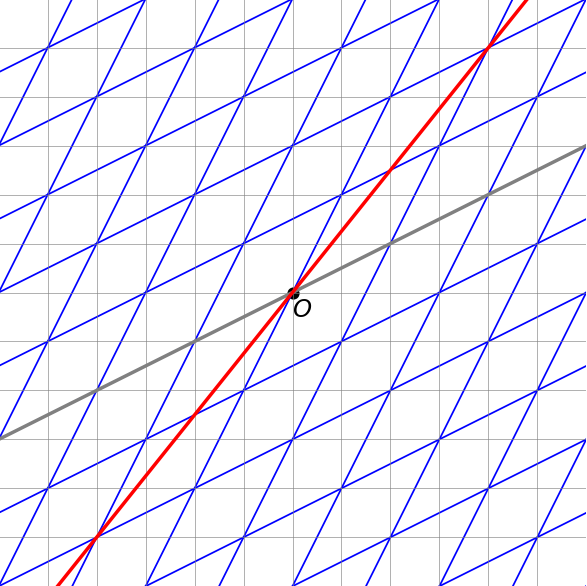
\includegraphics[width=7cm, height=5cm]{Slides/Figure/LT1.png}
    \end{figure}
 \[\mathbf{A}=\begin{bmatrix}
        1&2\\2&1
    \end{bmatrix}\]
\end{frame}
\begin{frame}
    \frametitle{Tiêu chí cho hình ảnh của lưới cho một phép biến đổi tuyến tính}
    \begin{itemize}
    \item Điểm O giữa nguyên vị trí.
    \item Các đường kẻ của lưới song song và cách đều nhau.
    \item Một đường thẳng vẫn là một đường thẳng.
\end{itemize}
\begin{figure}[H]
        \centering
        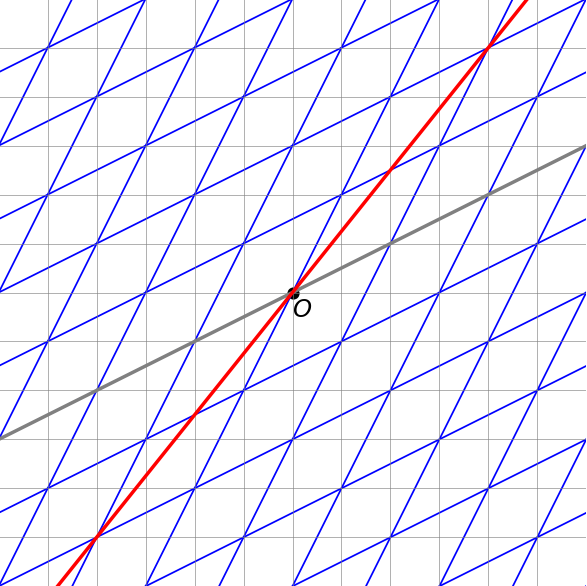
\includegraphics[width=6cm, height=4cm]{Slides/Figure/LT1.png}
    \end{figure}
\end{frame}
\begin{frame}
    \frametitle{Minh hoạ cho một phép biến đổi tuyến tính}
    \[\mathbf{v}=\begin{bmatrix}
    1\\0.5
\end{bmatrix}\rightarrow L\rightarrow L(\mathbf{v})=\begin{bmatrix}
    2\\2.5
\end{bmatrix}.\]
    \begin{figure}[H]
        \centering
        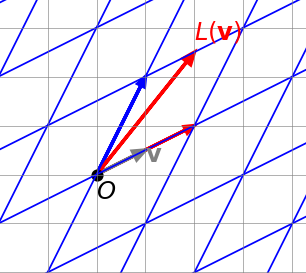
\includegraphics[width=6cm, height=4cm]{Slides/Figure/LT2.png}
    \end{figure}
\end{frame}
\begin{frame}
    \frametitle{Phép biến đổi cắt}
    \[\mathbf{A}=\begin{bmatrix}
        1&2\\0&1
    \end{bmatrix}\]
    \begin{figure}
        \centering
        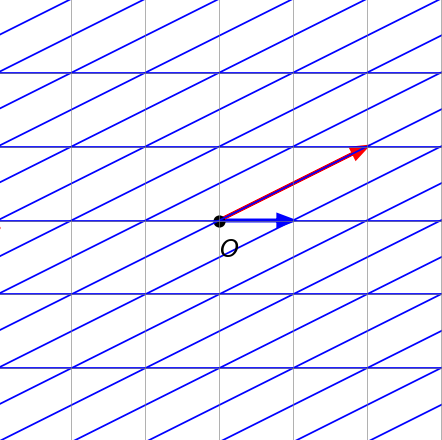
\includegraphics[width=5cm, height=4cm]{Slides/Figure/LT3.png}
    \end{figure}
\end{frame}
\begin{frame}
    \frametitle{Phép biến đổi cắt}
    Phương trình cho một biến đổi cắt 2D :
\[
L\left(\begin{bmatrix}
    x_1 \\x_2
 \end{bmatrix}\right)=\begin{bmatrix}
    x_1 +\lambda x_2 \\x_2
 \end{bmatrix}, \text{ hoặc}\quad 
 \begin{bmatrix}
    x_1 \\\lambda x_1 +x_2
 \end{bmatrix}.\]
Ma trận biến đổi đặc trưng
\[\begin{bmatrix}
    1&\lambda\\0&1
\end{bmatrix},\] hoặc 
\[\begin{bmatrix}
    1&0\\\lambda&1
\end{bmatrix}.\]
\end{frame}
\begin{frame}
    \frametitle{Phép giãn nở}
    \[\mathbf{D}=
    \begin{bmatrix}
        3&0\\0&5
    \end{bmatrix}\]
    \begin{figure}
        \centering
        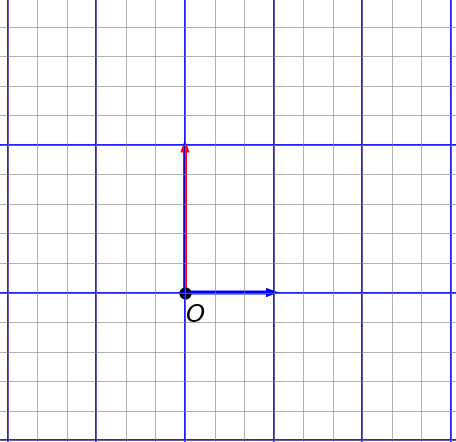
\includegraphics[width=5cm, height=4cm]{Slides/Figure/LT6.png}
    \end{figure}
\end{frame}
\begin{frame}
\frametitle{Phép giãn nở}
    Biến đổi cho một giãn nở 2D là 
\[L\left(\begin{bmatrix}
    x_1 \\x_2
\end{bmatrix}\right)=\begin{bmatrix}
    \lambda_1 x_1 \\\lambda_2 x_2
\end{bmatrix}.\]
Ma trận biến đổi là một ma trận đường chéo:
\[\mathbf{D}=\begin{bmatrix}
    \lambda_1 &0\\0&\lambda_2
\end{bmatrix}.\]
Chú ý, \[\mathbf{D}^{-1}=\begin{bmatrix}
    \lambda_{1}^{-1} &0\\0&\lambda_{2}^{-1}
\end{bmatrix}.\]
\end{frame}
\begin{frame}
    \frametitle{Phép quay}
    \begin{figure}[H]
        \centering
        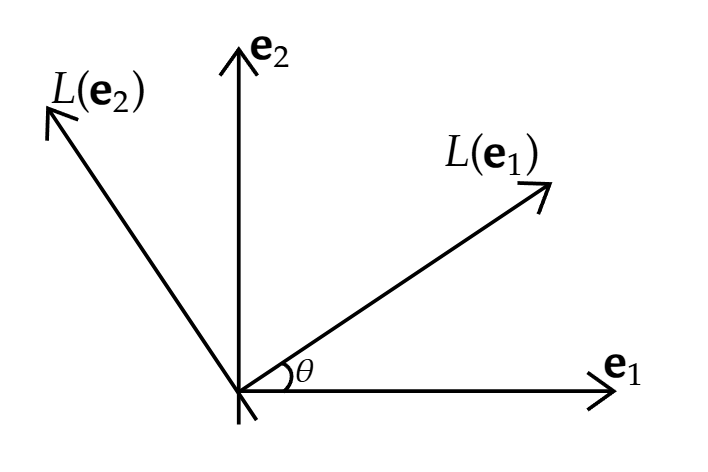
\includegraphics[width=6cm, height=4cm]{Slides/Figure/rotation.png}
    \end{figure}
    \[\mathbf{R}=\begin{bmatrix}
    \cos\theta &-\sin\theta\\
    \sin\theta &\cos\theta
\end{bmatrix};\qquad \mathbf{R}^{-1}=\mathbf{R}^T .\]
\end{frame}
\begin{frame}
    \frametitle{Phép quay}
    \begin{columns}
        \begin{column}{0.5\textwidth}
            \begin{figure}[H]
                \centering
                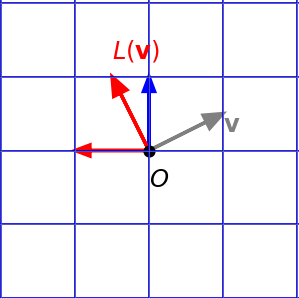
\includegraphics[width=3cm, height=3cm]{Slides/Figure/LT7.png}
            \end{figure}
            Phép quay 90 độ theo chiều dương
            \[\mathbf{R}=\begin{bmatrix}
                0&-1\\1&0
            \end{bmatrix}.\]
        \end{column}
        \begin{column}{0.5\textwidth}
            \begin{figure}[H]
                \centering
                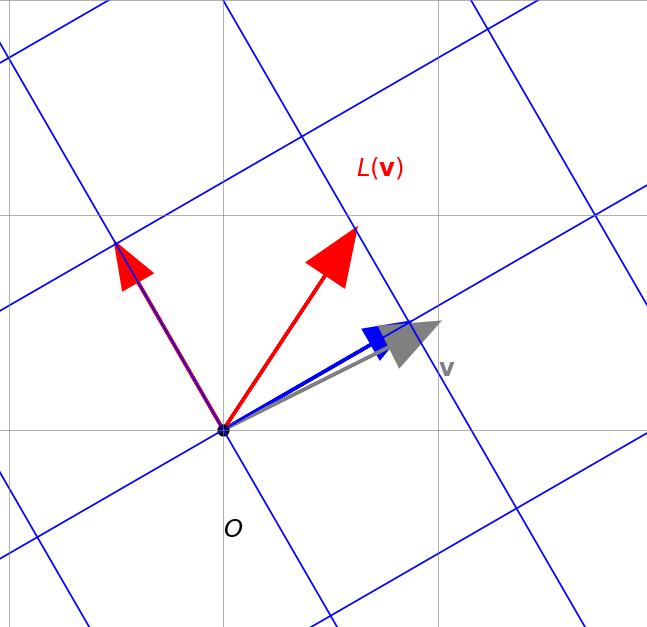
\includegraphics[width=3cm, height=3cm]{Slides/Figure/LT8.png}
            \end{figure}
            Phép quay 30 độ theo chiều dương
        \end{column}
    \end{columns}
\end{frame}
\begin{frame}
    \frametitle{Phép quay}
    \begin{figure}[H]
        \centering
        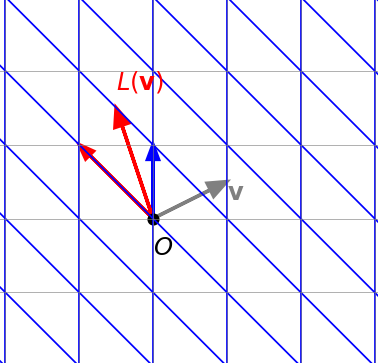
\includegraphics[width=5cm, height=4cm]{Slides/Figure/LT9.png}
    \end{figure}
    Kéo rồi quay 90 độ:
    \[\begin{bmatrix}
        0&-1\\1&0
    \end{bmatrix}\begin{bmatrix}
        1&1\\0&1
    \end{bmatrix}.\]
\end{frame}
\subsection{Chuyển cơ sở}
\begin{frame}
    \frametitle{Chuyển cơ sở}
    \begin{columns}
        \begin{column}{0.5\textwidth}
            Hai hệ cơ sở:
               \begin{itemize}
                  \item Hệ \(\mathcal{A}:\{\mathbf{e}_1 ,\mathbf{e}_2\}\) 
                \item Hệ \(\mathcal{B}:\{\mathbf{e}_3 ,\mathbf{e}_4\}\) 
                \end{itemize}
    Trong hệ \(\mathcal{A}\), \[\mathbf{v}_{\mathcal{A}}=\begin{bmatrix}
    5\\3
\end{bmatrix}.\] Trong hệ \(\mathcal{B}\), \[\mathbf{v}_{\mathcal{B}}=\begin{bmatrix}
    1\\3
\end{bmatrix}.\]
        \end{column}
        \begin{column}{0.5\textwidth}
            \begin{figure}
                \centering
                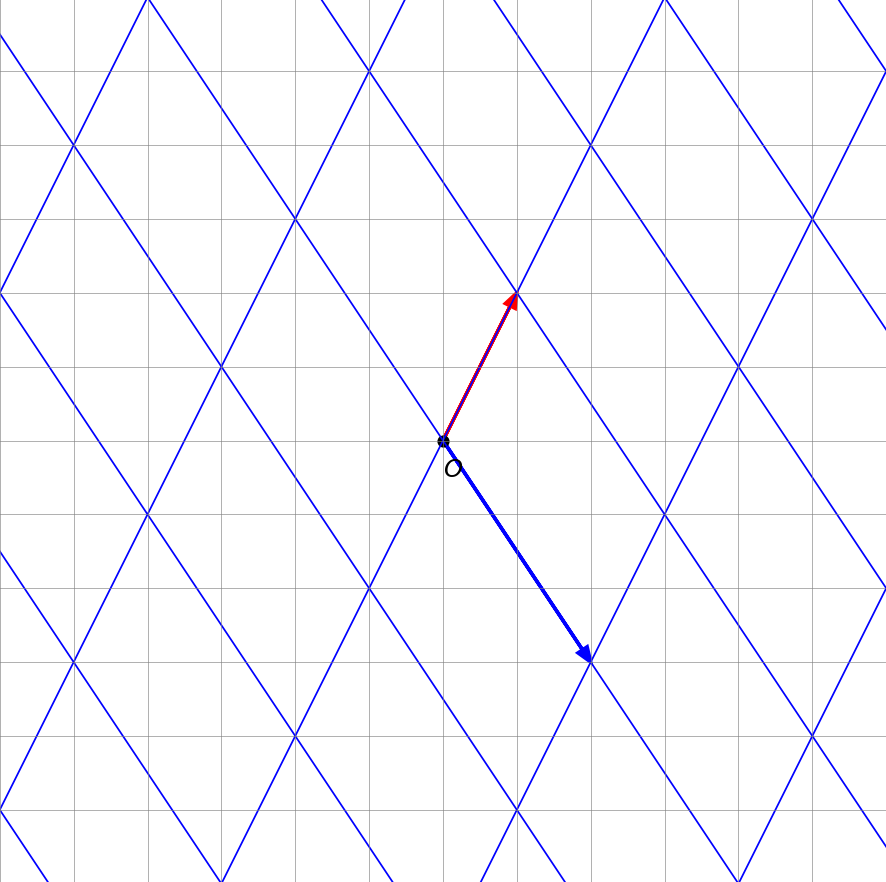
\includegraphics[width=7cm, height=5cm]{Slides/Figure/LT10.png}
            \end{figure}
        \end{column}
    \end{columns}
\end{frame}
\begin{frame}
    \frametitle{Chuyển cơ sở}
    \begin{columns}
        \begin{column}{0.5\textwidth}
            Biết rằng
           \[\mathbf{e}_3 =2\mathbf{e}_1 +(-3)\mathbf{e}_4 ,\quad \mathbf{e}_4 =1\mathbf{e}_1 +2\mathbf{e}_2 .\]
           Ta thu được gì?
          \[\begin{bmatrix}
    2&1\\-3&2
\end{bmatrix}\begin{bmatrix}
    1\\3
\end{bmatrix}=\begin{bmatrix}
    5\\3
\end{bmatrix},\] tức là
\[\mathbf{P}\mathbf{v}_{\mathcal{B}}=\mathbf{v}_{\mathcal{A}}.\]
        \end{column}
        \begin{column}{0.5\textwidth}
            \begin{figure}
                \centering
                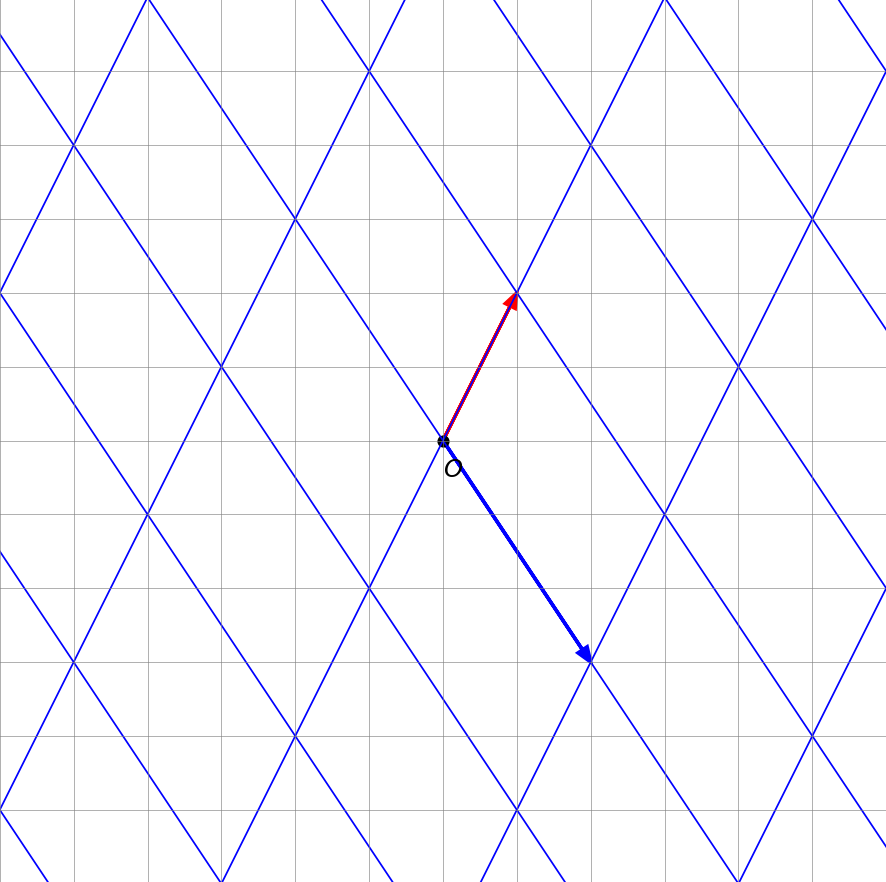
\includegraphics[width=7cm, height=5cm]{Slides/Figure/LT10.png}
            \end{figure}
        \end{column}
    \end{columns}
\end{frame}
\begin{frame}
    \frametitle{Chuyển cơ sở}
    \begin{columns}
        \begin{column}{0.5\textwidth}
        

          \[\mathbf{P}(\mathbf{e}_1)_{\mathcal{A}}=\mathbf{P}(\mathbf{e}_3)_{\mathcal{B}}=(\mathbf{e}_3)_{\mathcal{A}},\]
\[\mathbf{P}(\mathbf{e}_2)_{\mathcal{A}}=\mathbf{P}(\mathbf{e}_4)_{\mathcal{B}}=(\mathbf{e}_4)_{\mathcal{A}}.\] 
        \end{column}
        \begin{column}{0.5\textwidth}
            \begin{figure}
                \centering
                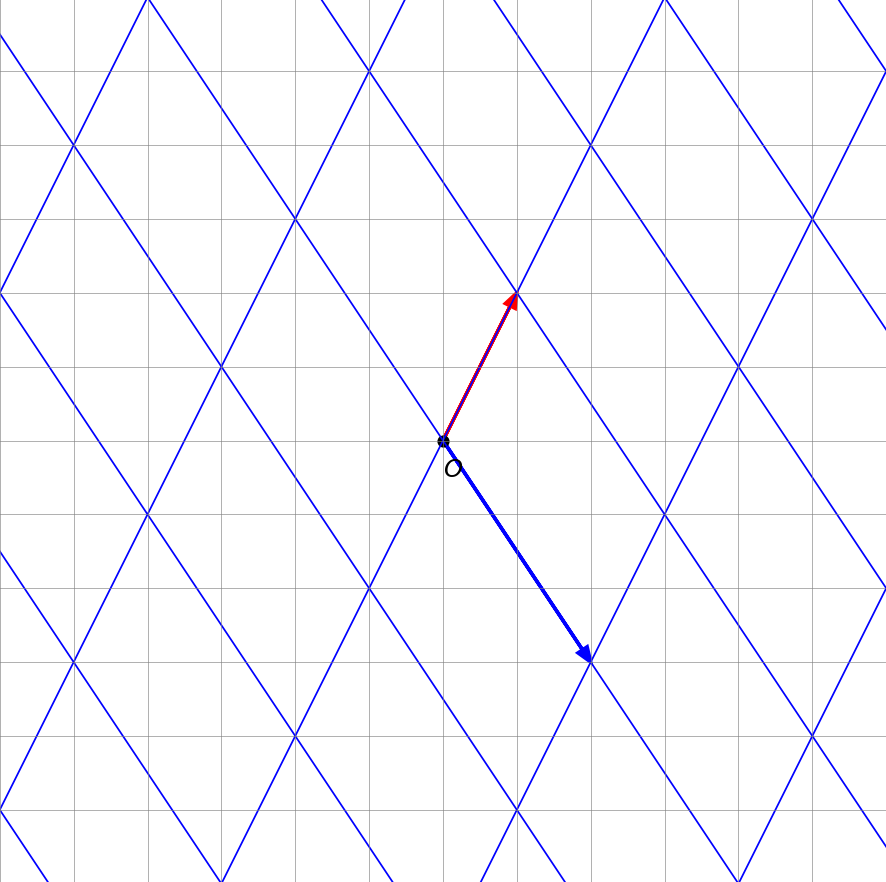
\includegraphics[width=7cm, height=5cm]{Slides/Figure/LT10.png}
            \end{figure}
        \end{column}
    \end{columns}
\end{frame}
\begin{frame}
    \frametitle{Chuyển cơ sở}
            \begin{equation*}
                \mathbf{P}\mathbf{v}_{\mathcal{B}}=\mathbf{v}_{\mathcal{A}}.
            \end{equation*}
        \begin{equation*}
            \mathbf{P}^{-1}\mathbf{v}_{\mathcal{A}}=\mathbf{v}_{\mathcal{B}}.
        \end{equation*}
                \begin{figure}[H]
        \centering
        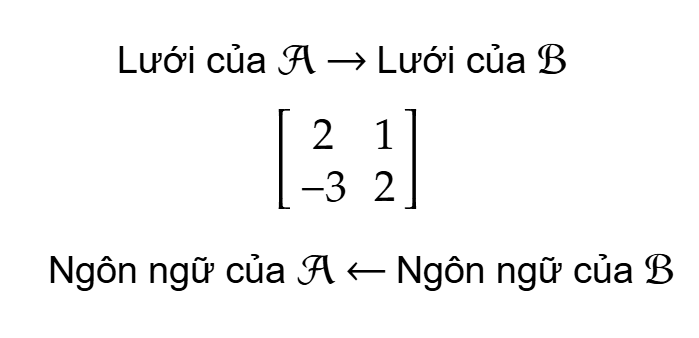
\includegraphics[width=7cm, height=4cm]{Slides/Figure/final.png}
    \end{figure}

\end{frame}
\begin{frame}
    \frametitle{Ví dụ}
    Một đường tròn bán kính \(R\) lăn không trượt với tốc độ không đổi, nghĩa là toạ độ của tâm đường tròn được cho bởi \((R\theta,R)\). Hãy xác định toạ độ của điểm M trong hệ toạ độ \(Oxy\), biểu diễn kết quả theo tham số \(\theta\).
\begin{figure}[H]
    \centering
    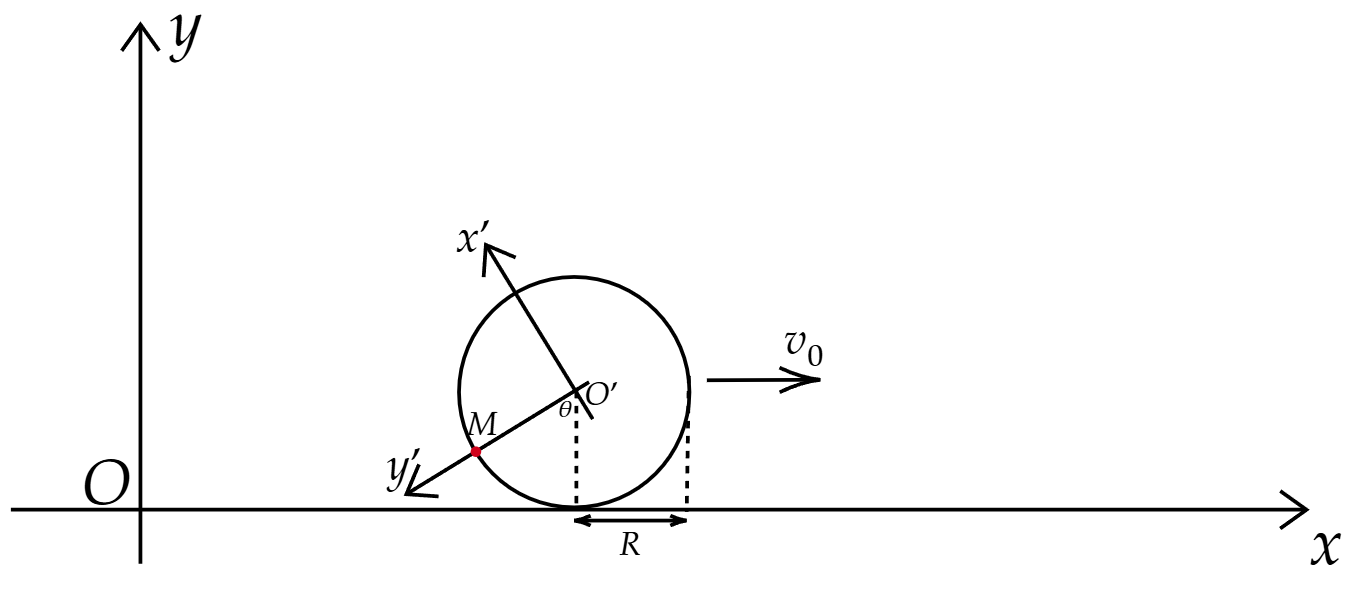
\includegraphics[width=9cm, height=4cm]{Slides/Figure/cycloidexample.png}
\end{figure}
\end{frame}
\begin{frame}
    \frametitle{Giải}
\[\begin{bmatrix}
    x\\y
\end{bmatrix}=\begin{bmatrix}
    \cos\phi&-\sin\phi \\\sin\phi&\cos\phi
\end{bmatrix}\begin{bmatrix}
    x'\\y'
\end{bmatrix}+\begin{bmatrix}
    R\theta\\R
\end{bmatrix},\] với \(\phi=\pi-\theta.\) Như vậy, 
\[\begin{bmatrix}
    x\\y
\end{bmatrix}=R\begin{bmatrix}
    \theta-\sin\theta\\1-\cos\theta
\end{bmatrix}.\] Quỹ đạo của điểm M chính là đường Cycloid.
\end{frame}
